\documentclass[a4paper, 10pt]{article}
\usepackage[utf8]{inputenc}
\usepackage{verbatim}
\usepackage{listings}
\usepackage{graphicx}
\usepackage{a4wide}
\usepackage{color}
\usepackage{amsmath}
\usepackage{amssymb}
\usepackage[dvips]{epsfig}
\usepackage[toc,page]{appendix}
\usepackage[T1]{fontenc}
\usepackage{cite} % [2,3,4] --> [2--4]
\usepackage{shadow}
\usepackage{hyperref}
\usepackage{titling}

\setlength{\droptitle}{-10em}   % This is your set screw

\setcounter{tocdepth}{2}

\lstset{language=c++}
\lstset{alsolanguage=[90]Fortran}
\lstset{basicstyle=\small}
\lstset{backgroundcolor=\color{white}}
\lstset{frame=single}
\lstset{stringstyle=\ttfamily}
\lstset{keywordstyle=\color{red}\bfseries}
\lstset{commentstyle=\itshape\color{blue}}
\lstset{showspaces=false}
\lstset{showstringspaces=false}
\lstset{showtabs=false}
\lstset{breaklines}
\title{FYS3150 - Project 1}
\author{Daniel Heinesen, Halvard Sutterud, Gunnar Lange}
\begin{document}
\maketitle
\begin{abstract}In this project we will study speed and numerical precision of
    linear algebra algorithms. Given a tridiagonal matrix, we use both a
    general solving algorithm for tridiagonal matrices and a special
    tailored method for our specific problem. This is also
    compared to a cumbersome LU-decomposition of the matrix.\\
    \linebreak
    Using an analytic expression for the diagonal elements in our special
    case, we were able to reduce the total number of FLOPS down to a total
    of $4n-3$ computations, where $n$ is the number of row and column
    elements in our matrix. 

    

\end{abstract}
\tableofcontents



\section{Introduction }
We solve the one-dimensional Poisson equation with Dirichlet boundary conditions by reducing it to a set of equations on the form of a tridiagonal matrix. This will transform a differential equation problem to a linear algebra problem. We wish to investigate different approaches to this linear algebra problem, and scrutinize their efficiency. To do this, we introduce three different methods for solving such linear algebra problems; the well-known LU-decomposition algorithm, applicable to any matrix, a general algorithm for solving tridiagonal matrices and finally an algorithm which takes into account the special features of the tridiagonal matrix we consider. As each of these algorithms is more specified than the previous, we can use more and more features intrinsic to our problem. This means that we can optimize the code, by pre-computing known, constant, quantities.\\
\linebreak
We begin by introducing the theoretical model, and presenting the selected algorithms. We then provide a brief overview of the implementation of these methods, and some points to be cautious of. Subsequently, we present our results and discussion thereof. Finally we discuss the overarching conclusion that may be drawn from this project, and suggest some possible future direction for this research.

\section{Theoretical model}\label{Theoretical_section}
\subsection{Discretizing the Poisson equation}\label{Discretize_Poisson}
Assume that $u(x)$ is a four-times differentiable function, $u(x) \in C^4$. Using Taylor polynomial up the the fourth degree, a general approximation formula to the second derivative can be derived as:
\begin{equation}\label{eq:continuous_derivative}
\frac{d^2 u}{dx^2}\approx \frac{u(x+h)+u(x-h)-2u(x)}{h^2}+O(h^2)
\end{equation}
This formula is derived in appendix \ref{appendix_A}. Discretizing $u(x)$ at points $x_1, x_2, ..., x_n$, and  introducing the convenient notation $u(x_i)=u_i$, this formula can be rewritten in discrete form as:
\begin{equation}\label{eq:discrete_Poisson}
\frac{d^2 u}{dx^2}\approx \frac{u_{i+1}+u_{i-1}-2u_{i}}{h^2}+O(h^2)
\end{equation}
Where $h$ is the distance between the grid points, given by $h=1/(n+1)$. If one additionally imposes Dirichlet boundary conditions, i.e. that $u_0=u_{n+1}=0$, this formula is valid for all $x_i$, $i\in [1, n]$. Inserting this formula into the Poisson equation with right-hand side $f(x)$, and letting $f(x_i)=f_i$, gives:
\begin{equation}\label{Poisson}
-\frac{u_{i+1}+u_{i-1}-2u_{i}}{h^2}=f_i
\end{equation}\label{Poisson}
This can be rephrased as a linear algebra problem, of the form:
$$\mathbf{A}\mathbf{u}=h^2\mathbf{f}$$
Where $\mathbf{A}$ is a $n \times n$ given by:
$$\mathbf{A}=\begin{pmatrix}
2 & -1 & 0 & \ldots &  \ldots & 0\\
-1 & 2 & -1  & 0 & \ldots & 0\\
0 & -1 & 2 &-1 & 0 & \ldots \\
0 & 0 & -1 & 2 &-1 &\ldots\\
\vdots &  & &  &\ddots & \vdots \\
0 && \ldots && -1&  2  \\
\end{pmatrix}$$
Notice that $\mathbf{A}$ is a tridiagonal matrix. This makes the general solution algorithm much simpler.
\subsection{Solving a general tridiagonal matrix problem}\label{general_algorithm_section}
A general tridiagonal matrix problem can be written as:
$$\begin{pmatrix}
a_{1} & b_1 & 0 & \ldots &  \ldots & 0\\
c_1 & a_2 & b_2  & 0 & \ldots & 0\\
0 & c_2 & a_3 &b_3 & 0 & \ldots \\
0 & 0 & c_3 & a_4 &b_4 &\ldots\\
\vdots &  & &  &\ddots & \vdots \\
0 && \ldots && c_{n-1}&  a_n  \\
\end{pmatrix}\begin{pmatrix}
u_1\\
u_2\\
u_3\\
u_4\\
\vdots\\
u_n\\
\end{pmatrix}=\begin{pmatrix}
v_1\\
v_2\\
v_3\\
v_4\\
\vdots\\
v_n
\end{pmatrix}$$
Where, in the specific case above, $v_n=f_n/h^2$. This problem may be solved in two steps: a decomposition and forward substitution, and a backward substitution. The goal is to make each column a pivot column. For the forward substitution, it is easiest to first transform the matrix into an upper-diagonal matrix. Thus, $c_1$ needs to be zero. This can be achieved by subtracting $c_1/a_1$ times the first row from the second row. This gives:
$$\begin{pmatrix}
a_{1} & b_1 & 0 & \ldots &  \ldots & 0\\
0 & \tilde{a_2} & b_2  & 0 & \ldots & 0\\
0 & c_2 & a_3 &b_3 & 0 & \ldots \\
0 & 0 & c_3 & a_4 &b_4 &\ldots\\
\vdots &  & &  &\ddots & \vdots \\
0 && \ldots && c_{n-1}&  a_n  \\
\end{pmatrix}\begin{pmatrix}
u_1\\
u_2\\
u_3\\
u_4\\
\vdots\\
u_n\\
\end{pmatrix}=\begin{pmatrix}
v_1\\
\tilde{v_2}\\
v_3\\
v_4\\
\vdots\\
v_n
\end{pmatrix}$$
Where:
$$\tilde{a_2}=a_2-\frac{c_1}{a_1}b_1, \quad \tilde{v_2}=v_2-\frac{c_1}{a_1}v_1$$
Notice how only $a$ and $v$ changes in this step. Thus all parameters will be the same in the next time step, but the $a$ and $v$ from the previous time step, will now be $\tilde{a}$ and $\tilde{v}$. It is therefore easy to generalize the above formulae to:
\begin{equation}\label{eq:forward_substitution_1}
\tilde{a}_{i+1}=a_{i+1}-\frac{c_ib_i}{\tilde{a_i}}
\end{equation}
\begin{equation}\label{eq:forward_substitution_2}
\tilde{v}_{i+1}=v_{i+1}-\frac{c_i}{\tilde{a_i}}\tilde{v_i}
\end{equation}
These equations can now be iterated from $i=1$ to $n-1$. We then end up with an upper triangular matrix, containing $\tilde{a_i}$ and $b_i$, given by:
$$\begin{pmatrix}
a_{1} & b_1 & 0 & \ldots &  \ldots & 0\\
0 & \tilde{a}_2 & b_2  & 0 & \ldots & 0\\
0 & 0 & \tilde{a}_3 &b_3 & 0 & \ldots \\
0 & 0 & 0 & \tilde{a}_4 &b_4 &\ldots\\
\vdots &  & &  &\ddots & \vdots \\
0 && \ldots && 0&  \tilde{a}_n  \\
\end{pmatrix}\begin{pmatrix}
u_1\\
u_2\\
u_3\\
u_4\\
\vdots\\
u_n\\
\end{pmatrix}=\begin{pmatrix}
v_1\\
\tilde{v}_2\\
\tilde{v}_3\\
\tilde{v}_4\\
\vdots\\
\tilde{v}_n
\end{pmatrix}$$
Now we need a $1$ in the last entry of the matrix. This is easily achieved by dividing by $\tilde{a}_n$. The other pivot elements can be obtained by backwards substitution, by employing the following algorithm. 
\begin{itemize}
\item Subtracting $b_i$ times the $i+1$th row from the $i$th row (because the $i+1$th row will have a $1$ as a pivot).
\item Divide the $i$th row by $\tilde{a_i}$
\end{itemize}
This will impact the $\tilde{v}_i$, converting them into $w_i$, according to:
\begin{equation}\label{eq:backwards_substitution}
w_i=\frac{\tilde{v}_i-b_iw_{i+1}}{\tilde{a_i}}
\end{equation}
This defines a general algorithm for solving a tridiagonal matrix problem. The efficiency of this algorithm is surprisingly easy to calculate, as shown in the next section.
\subsection{Counting the number of FLOPS}
The general algorithm consists of equations \ref{eq:forward_substitution_1}, \ref{eq:forward_substitution_2} and \ref{eq:backwards_substitution}. Let us look at the required FLOPS for each of these equations:
\paragraph*{Equation \ref{eq:forward_substitution_1}}
This equation requires the computation of $x=c_i/\tilde{a}_{i}$. After this, we compute $y=x\cdot b_i$, and finally the computation $z=a_{i+1}-y$. This is done for $n-1$ points (as it is not required for the first row), giving a total of $3(n-1)$ FLOPS for this equation.
\paragraph*{Equation \ref{eq:forward_substitution_2}}
This equation requires the computation of $x=c_i/\tilde{a}_i$, but this has already been computed in the previous step, and therefore does not require additional FLOPS. Then, we need to compute $y=x\tilde{v_i}$ and finally $z=v_{i+1}-y$. This therefore requires a total of $2(n-1)$ FLOPS.
\paragraph*{Equation \ref{eq:backwards_substitution}}
This equation requires the computation of $x=b_iw_{i+1}$, followed by the computation of $y=\tilde{v}_i-x$, and finally the computation $z=y/\tilde{a}_i$. This gives a total of $3(n-1)$ FLOPS.
\paragraph*{Total}
Thus totally, the algorithm requires $8(n-1)$ FLOPS. However, we have ignored the division by $\tilde{a_n}$ to get $w_n$. This requires one additional FLOP, giving the total number of FLOPS as:
$$\mathrm{FLOPS}=8n-7$$
\subsection{Tailoring an algorithm}\label{tailored_algorithm_section}
In the previous sections, we have developed and analyzed an algorithm for a general tridiagonal matrix. However, as seen from equation 1, the matrix in our case is significantly simpler. This comes from the fact that there are only three distinct numbers present in our matrix. This means that \textit{all quantities} which only require $a_i$, $b_i$ or $c_i$ can be computed a priori. It is also possible to obtain an analytic expression for $\tilde{a}_i$, as follows.
\paragraph*{Finding an analytical expression for $\tilde{a}_i$}: The general formula for $\tilde{a}_{i+1}$ is given by equation \ref{eq:forward_substitution_1}. In our case, $c_i=b_i=-1$ and $a_{i+1}=2$. Thus equation \ref{eq:forward_substitution_1} can be rewritten as:
\begin{equation}\label{eq:forward_substitution_tailored}
\tilde{a}_{i+1}=2+\frac{1}{\tilde{a}_i}
\end{equation}
Note that $\tilde{a}_1=a_1=2$. Trying out some iterations, it seems that:
\begin{equation}\label{eq:general_an}
\tilde{a}_{i+1}=-\frac{(i+2)}{i+1}
\end{equation}
This is proved in appendix \ref{appendix_B}. Thus, $\tilde{a}_i$ can also be pre-computed. This means that the number of FLOPS during runtime can be significantly reduced.
\newpage
\subsection{Countinger the number of FLOPS in the tailored algorithm}
\paragraph{Equation \ref{eq:forward_substitution_1}} This can be pre-computed, and therefore does not contribute any FLOPS during runtime. 
\paragraph*{Equation \ref{eq:forward_substitution_2}} As $\tilde{a}_i$ is already pre-computed, we can also pre-computed $\tilde{a}_i^{-1}$. Thus this equation only requires the multiplication of $x=\tilde{v_i}\frac{c_i}{\tilde{a}_i}$, followed by the subtraction $y=v_{i+1}-x$, for a total of $2(n-1)$ FLOPS. 
\paragraph*{Equation \ref{eq:backwards_substitution}} Here we only need to compute $x=\tilde{v}_i+w_{i+1}$ (since $b_i=-1$), followed by the computation $x/\tilde{a}_i$ for a total of $2(n-1)$ FLOPS. 
\paragraph*{Total}
This gives a total of $4n-4$ FLOPS. However, we still need to compute $\tilde{v}_n/a_n$ as well, which gives on additional FLOP, for a total of:
$$\mathrm{FLOPS}=4n-3$$
Which approximately cuts the running time by a factor 2. 
\subsection{Comparing with LU-decomposition}
Another common algorithm for solving a set of matrix equations (effectively inverting the marix) is LU-decomposition. This is a process which decomposes any initial matrix, $\mathbf{A}$ to a product of an upper triangular ("$\mathbf{U}$") and a lower triangular ("$\mathbf{L}$") matrix, i.e:
\begin{equation}
\mathbf{A}=\mathbf{L}\mathbf{U}
\end{equation}
This is useful because the matrix equation $\mathbf{A}\mathbf{x}=\mathbf{b}$ can now be rewritten as:
$$\mathbf{L}\mathbf{U}\mathbf{x}=\mathbf{b}$$
Which can be solved as:\\
\begin{equation}\label{eq:LU_1}
\mathbf{L}\mathbf{y}=\mathbf{b}
\end{equation}
\begin{equation}\label{eq:LU_2}
\mathbf{Ux}=\mathbf{x}
\end{equation} These equations are significantly easier to solve than the original problem, as the matrices involved are now triangular.\\
\linebreak This algorithm has been analyzed thoroughly in the literature, see for example \cite{LU-decomp}. As proved there, the algorithm is of order $(2/3)n^3$. 
\subsection{The specific problem and its analytic solution} \label{analytic_solution}
In this paper we will investigate the solution to the following special case of Poisson's equation:
\begin{equation}\label{eq:poisson_rhs}
-\frac{d^2 u}{dx^2}=100e^{-10x}
\end{equation}
With Dirichlet boundary conditions on the intervanl $x\in [0, 1]$. The main motivation for choosing this specific right-hand side is that the analytic solution is relatively easy to obtain. Simply integrating twice gives:
$$u(x)=-e^{-10x}+A+Bx$$
Requiring that $u(0)=u(1)=0$ gives, after some algebra, the analytic solution as:
\begin{equation}\label{eq:analytic_solution}
u(x)=1-(1-e^{-10})x-e^{-10x}
\end{equation}
\section{Method}\label{Method}
All programs and benchmarks calculations can be found on our \href{https://github.com/dulte/Comp-Phys/tree/master/Project1}{GIT repository}\footnote{https://github.com/dulte/Comp-Phys/tree/master/Project1}. All these calculations were timed, using the module found in \cite{Morten}
\subsection{Implementing the general algorithm}
This algorithm consists of two loops: the decomposition and forward substitution, followed by the backwards substitution, as discussed in section \ref{general_algorithm_section}. In Pseudo-Code:
\lstinputlisting{Pseudo_code_1.cpp}
Note how this code does not assume anything about the tridiagonal matrix, and can thus be used for a general tridiagonal matrix. This is just a numerical implementation of the equations from section \ref{Discretize_Poisson}. Note, however, that this algorithm does not take into account the boundary conditions. These must be added (simply as zeros at the extreme points of the vectors) separately. 
\subsection{Implementing the tailored algorithm}
The algorithm which is tailored to our problem is computationally lighter, as described in section \ref{tailored_algorithm_section}. It is also easier to implement, as a lot of the relevant quantities can be pre-computed. There are still two loops, but these are now significantly simpler, as shown in the Pseudo-code below:
\lstinputlisting{Pseudo_code_2.cpp} 
Where a\_inv=$a^{-1}$. Note that this algorithm only works if the input matrix is in the form discussed in section \ref{tailored_algorithm_section}. Note also that the comment from the previous section about the boundary condition applies.
\newpage
\subsection{Implementing the LU-Decomposition}
The LU-decomposition is implemented by means of the Armadillo Linear Algebra library for $C++$. This is done in two steps. First we initialize a matrix $\mathbf{A}$ (in this case a tridiagonal matrix, though it can be of any kind). Then we solve equations \ref{eq:LU_1} and \ref{eq:LU_2} by using Armadillo's \textit{solve} method . In Pseudo-Code:
\lstinputlisting{Pseudo_code_3.cpp} 
\subsection{Comparing the results to the analytic solution}\label{compare_error}
The analytic solution is rather straightforward to implement as a separate function. We tested our algorithms with multiple step-sizes $h$ (and therefore different $n$'s) to get a sense of how well it converges to the analytic solution derived in section \ref{analytic_solution}. A good measure of "closeness" to the analytic solution is the log of the relative error, as found in \cite{Morten}, defined by:
\begin{equation}\label{eq:relative_error}
\epsilon_i=\log_{10}\left(\left|\frac{v_i-u_i}{u_i}\right|\right)
\end{equation}
Where $u_i$ is the analytic solution at a specified point, and $v_i$ is the numerical solution at the same point. We will employ this expression to plot the relative error. Note that we only record the maximum error which occurs for a specific value of $n$.
\newpage
\section{Results and discussion}
\subsection{Convergence to the analytic solution}\label{Convergence_to_solution}
\subsubsection{Results}
At plot of the analytic solution versus a range of values for $n$ is shown in figure \ref{fig:figure_1} below. Note that $n$ denotes the number of points \textit{within} the tridiagonal matrix, so that the total number of points is $n+2$ (including the endpoints). Note also that this plot is independent of which of the methods discussed in section \ref{Theoretical_section} is used, as they are all based on the same discretization of the second derivative. The only difference between these methods is the CPU time required.\\
\begin{figure}[h!!]
\fbox{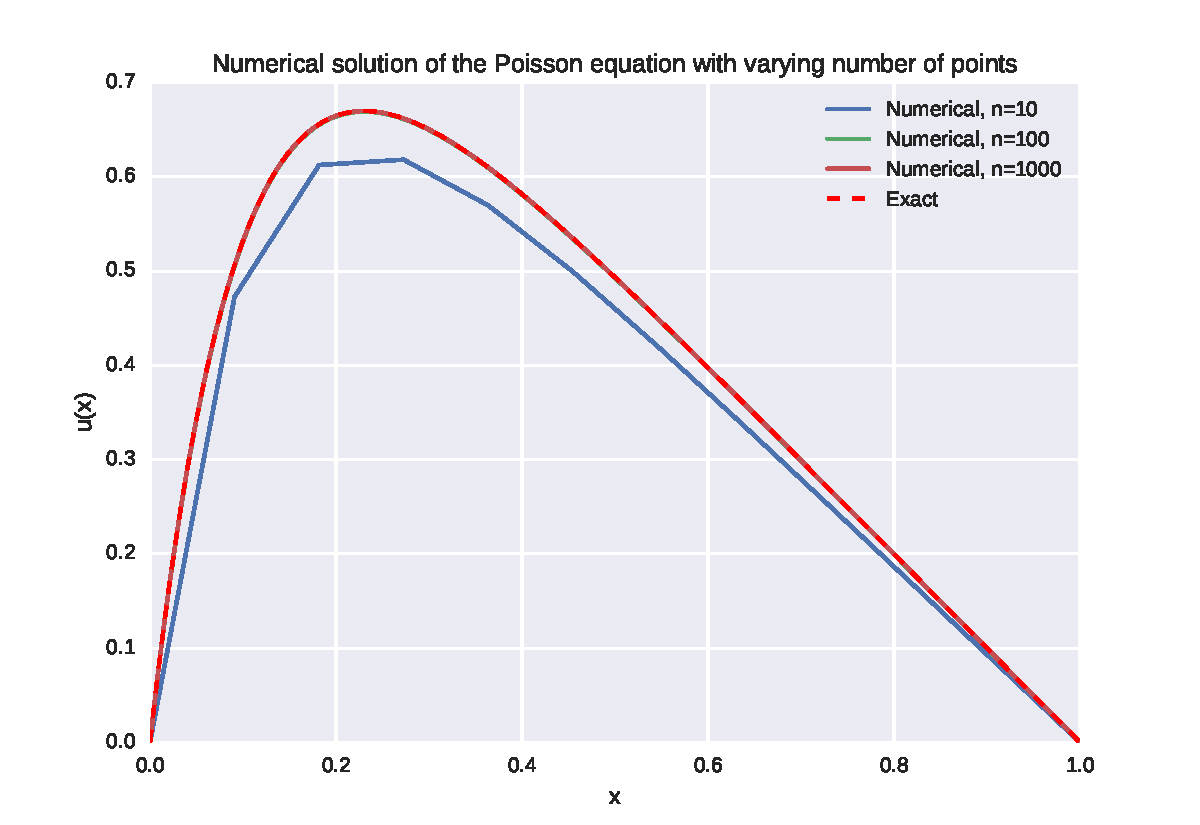
\includegraphics[scale=0.8]{Project1_general_algorithm.pdf}}
\caption{Plot of the solution, $u(x)$,  to the differential equation defined in equation
\ref{eq:poisson_rhs}. The dashed line is the analytic solution derived in section \ref{analytic_solution}. The other lines come from numerical simulations with a varying number of integration points, as described in section \ref{Method}}
\label{fig:figure_1}
\end{figure}
\newpage
\subsubsection{Discussion}
Clearly the methods converge rapidly, as predicted by the quadratic error term in equation \ref{eq:continuous_derivative}. A closer analysis of the error term is found in appendix \ref{appendix_A}. This shows that the mathematical (truncation) error of the second derivative of $u(x)$ at $a$ is given by:
\begin{equation}
O(h^2)= -\frac{h^2}{12}f^{(4)}(\xi), \quad \xi \in (a-h, a+h)
\end{equation}
Note the negative sign. Differentiating the analytical solution (equation \ref{eq:analytic_solution}) four times gives a strictly positive expression on the interval $x\in (0,1)$;
$$\frac{d^4 u}{dx^4}=10^4 e^{-10x}$$
And thus the error term will tend to make the numerical solution \textit{smaller} than the analytic solution. This is the behavior we can observe for $n=10$ in figure \ref{fig:figure_1}. Closer inspection of the plot reveals a similar behavior for larger values of $n$, as shown in figure \ref{fig:figure_2} below.
\begin{center}
\begin{figure}[h]
\fbox{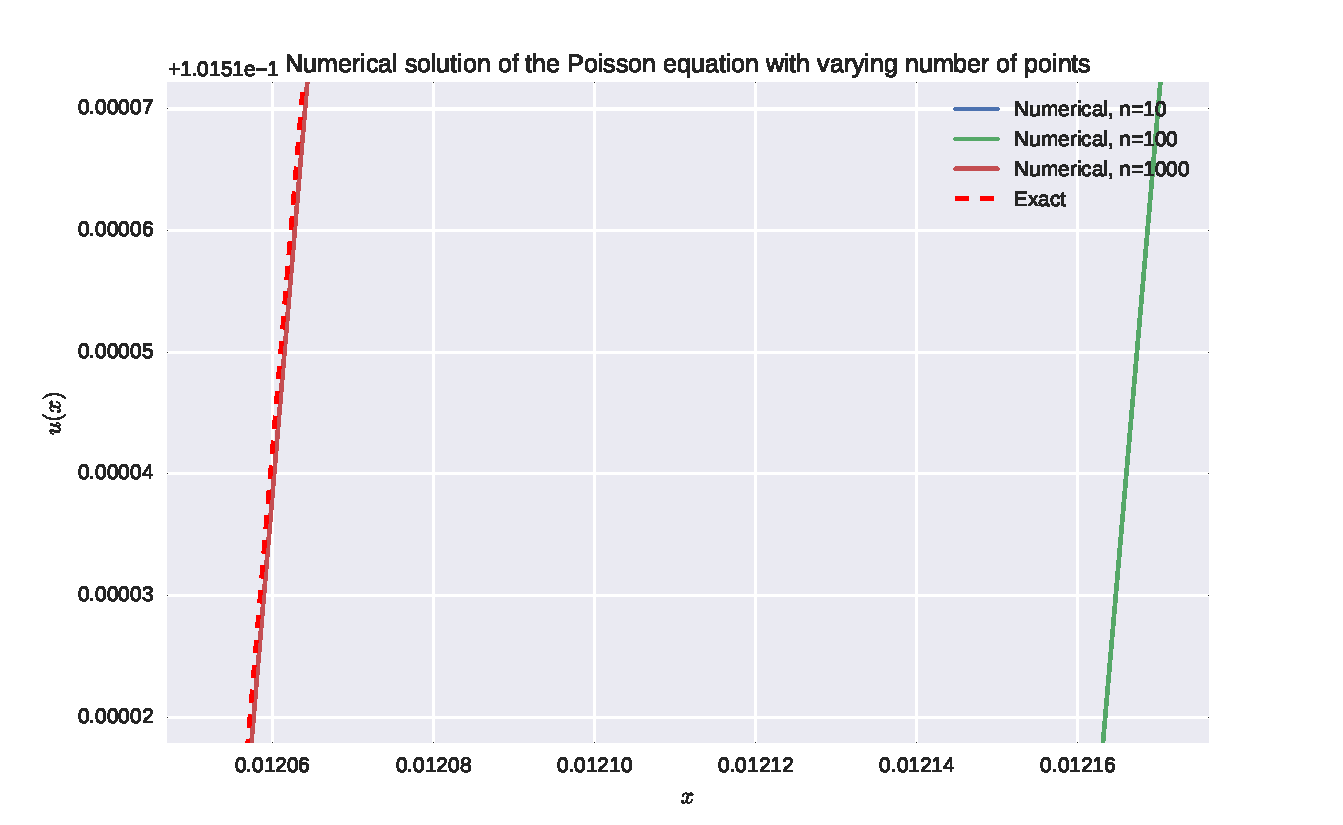
\includegraphics[scale=0.7]{project1_general_zoom.pdf}}
\caption{Zoomed in version of figure \ref{fig:figure_1}.} 
\label{fig:figure_2}
\end{figure}
\end{center}
\pagebreak
\subsection{Relative error}
\subsubsection{Results}
A log-log plot of the error, as described in section \ref{compare_error} is shown in figure \ref{fig:figure_3} below.
\begin{center}
\begin{figure}[h]
\fbox{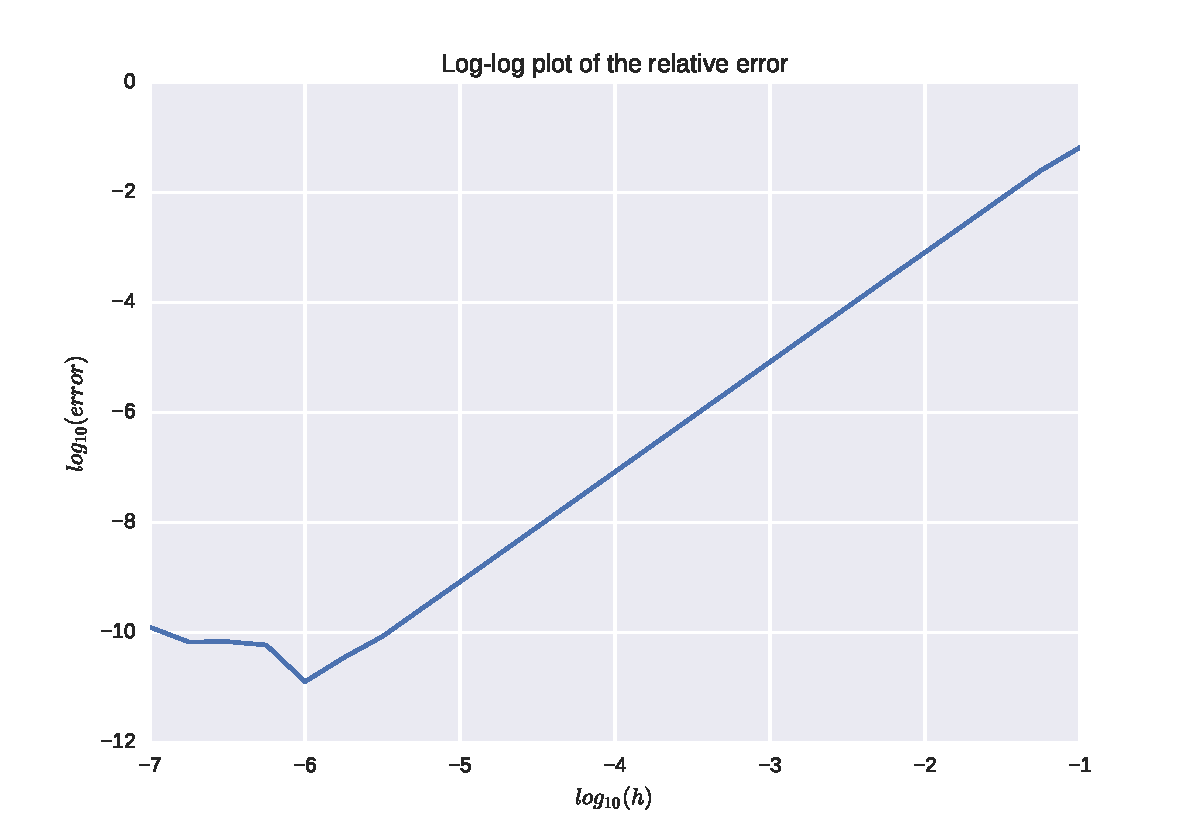
\includegraphics[scale=0.75]{Project1_log_error.pdf}}
\caption{Plot of relative error. $x$-axis is the step-size, $y$-axis is the relative error. The effect is a combination of truncation and round-off errors.} 
\label{fig:figure_3}
\end{figure}
\end{center}
\subsubsection{Discussion}
The error is composed of two components: a truncation error (as we used a finite step size) and a numerical (round-off) error. I have already investigated the truncation error of our method, and know that it decreases as a function of $h^2$. A close analysis of the round-off error is done in \cite{Morken}, where it is shown that the round-off error for the second-derivative at $a$ is given by:
\begin{equation}
\epsilon_{round-off} = \frac{3\epsilon^*}{h^2}f(\xi) \quad \xi \in (a-h, a+h)
\end{equation}
Here $\epsilon^*$ is the smallest possible distance between two floating points numbers (in the reference approximated as $\epsilon^* \approx 6\cdot 10^{-16}$. Thus there are two opposing factors contributing to the error - the truncation error is proportional to $h^2$, and decreases with decreasing step-size, whereas the numerical errors are proportional to $1/h^2$, and increase with decreasing step-size. Therefore, we would expect to reach a point where the increase in the round-off errors are larger than the decrease in the truncation errors, whereupon further increasing $n$ only increases the error. This is exactly what we observe.
\subsection{Comparison of computational speed}
\subsubsection{Results}
We compare the computational speed of the various algorithms described in section \ref{Theoretical_section} for a range of $n$-values in the table below:
\begin{table}[h]
\label{table1}
\begin{tabular}{|c|c|c|c|}
\hline
 \multicolumn{1}{|c|}{\textbf{Number of points, $\mathbf{n}$}} & 
  \multicolumn{3}{|c|}{\textbf{Time taken, $s$ (seconds)}} \\
\cline{2-4}
 & \textbf{General method} & \textbf{Tailored method} & \textbf{LU-decomposition} \\
\hline
$10^1$ & $2\cdot 10^{-6}$ & $2.0\cdot 10^{-6}$ & $2.2\cdot 10^{-3}$\\
$10^2$ & $7\cdot 10^{-6}$ & $5.0\cdot 10^{-6}$ & $1.6 \cdot 10^{-3}$\\
$10^3$ & $6.6\cdot 10^{-5}$ & $4.1\cdot 10^{-5}$ & $8.1\cdot 10^{-2}$\\
$10^4$ & $6.7\cdot 10^{-4}$ & $2.6\cdot 10^{-4}$ & $7.7$\\
$10^5$ & $6.6 \cdot 10^{-3}$& $3.0 \cdot 10^{-3}$& N/A\\
$10^6$ & $5.9\cdot 10^{-2}$ & $2.4 \cdot 10^{-2}$& N/A\\
$10^7$ & $6.6 \cdot 10^{-1}$ & $2.7 \cdot 10^{-1}$& N/A\\
\hline
\end{tabular}
\caption{Comparing time taken to compute a solution to the Poisson equation for a range of $n$ for the different algorithms described in \ref{Theoretical_section}}
\end{table}
\subsection{Discussion}
As expected (according to the theory in section \ref{Theoretical_section}), the tailored method is superior to the general method, which are both far superior to the LU-decomposition. Notice how the LU-decomposition fails after $n=10^5$, because there is not enough memory available.\\
\linebreak
One odd feature of the above table is that it takes \textit{more} time to LU-decompose a $10\times 10$ matrix than it takes to decompose a $100 \times 100$ matrix. Wilst both are relatively fast, they are extremely slow when compared to the other methods. It is not entirely obvious why this is the case, and this may be something worth investigating further.
\newpage

\section{Conclusion}
\subsection{Results of this project}
We have shown that, for a tridiagonal matrix problem, it is better to carefully consider the problem in advance, and utilize as many of the special, simplifying, properties as possible. We have also shown that proper optimization and specialization of the methods can open up the possibility to compute problems (such as solving this problem with $n=10^7$) which are not solvable by more general methods. We have also investigated numerical and round-off errors in our methods, and shown that they have opposing effects, which implies that, even if powerful CPU capabilities are available, the step size has to be chosen carefully.
\subsection{Future outreach}
One interesting aspect of our solution is that the LU-decomposition took longer time for a $10\times 10$  matrix than for a $100 \times 100$ matrix. This may just be an error in our program, but either way it is worth investigating further. Perhaps, one could only time the time it takes to compute the solution of the equation, and ignore the time it takes to build the required matrix. This may change the computational speed of the LU-decomposition, but it would still not enable it to work on matrices larger than $10^5 \times 10^5$.\\
\linebreak
 Whilst it seems unlikely that a large amount of optimization is possible for the tridiagonal matrix discussed here, it may be interesting to investigate methods to generalize this. One example would be matrices with more than two off-diagonal elements, or matrices with different structures (such as alternating elements along the off-diagonals). 

\begin{thebibliography}{9}
\bibitem{LU-decomp}
Marco Chiarandini.
\textit{LU Factorization}
\\\texttt{http://www.imada.sdu.dk/~marco/DM554/Slides/dm554-lu.pdf}

\bibitem{Morken}
Knut Mørken.
\textit{Numerical Algorithms and Digital Representation}
University of Oslo, Oslo, 2015.

\bibitem{Morten}
Morten Hjorth-Jensen.
\textit{Project1 - 2016}
Computational Physics Autumn 2016.
\\\texttt{https://github.com/CompPhysics/ComputationalPhysics/blob/gh-pages/doc/Projects}


\end{thebibliography}

\newpage
\begin{appendices}
\section{Deriving the error in the second derivative}\label{appendix_A}
We will here derive the formula for the truncation error in our approximation to the second derivative, as employed in section \ref{Discretize_Poisson} and \ref{Convergence_to_solution}.\\
\linebreak
Assume, as in section \ref{Discretize_Poisson}, that $u(x) \in C^4$. Using Taylor expansion, the function may be expanded around a point $a$ as:
$$f(a+h) = f(a)+hf'(a)+\frac{h^2}{2}f''(a)+\frac{h^3}{3!}f'''(a)+\frac{h^4}{4!}f^{(iv)}(\xi_1)$$
Where $\xi_1 \in [x-h, x+h]$. We can also expand the function the other way as:
$$f(a-h) = f(a)-hf'(a)+\frac{h^2}{2}f''(a)-\frac{h^3}{3!}f'''(a)+\frac{h^4}{4!}f^{(iv)}(\xi_2)$$
Where $\xi_2 \in [a-h, a+h]$. Adding these equations gives:
$$f(a+h)+f(a-h)=2f(a)+h^2f''(a)+\frac{h^4}{12}f^{(iv)}(\xi)$$
Where $\xi \in [a-h, a+h]$. Rearranging gives:
$$f''(a)=\frac{f(a+h)-2f(a)+f(a-h)}{h^2}-\frac{h^2}{12}f^{(iv)}(\xi)$$
Which is exactly equation \ref{eq:continuous_derivative}, where we have exchanged the error term with a general $O(h^2)$.
\section{Deriving the general formula for $a_n$}\label{appendix_B}
Here we are going to give a proof by induction for equation \ref{eq:general_an}, which was stated as:

$$
\tilde{a}_{i+1}=-\frac{(i+2)}{i+1}
$$


We begin by looking at $i=1$

$$
\tilde{a}_{2} = -2 + \frac{1}{2} = -\frac{3}{2} = -\frac{1+1}{1+2}
$$

So the hypothesis is correct for $i = 1$. We now define $k = i+1$, and proves that the hypothesis holds for $k+1$:

$$
\tilde{a}_{k+1} = -2 - \frac{1}{\tilde{a}_{k}} = -2 + \frac{k}{k+1}
$$

$$
= \frac{-2(k+1) + k}{k+1} = \frac{-k - 2}{k+1} = -\frac{k+2}{k+1}
$$

Which is the gives us the expected expression, and the hypothesis is proved.


\hfill $\blacksquare$
\end{appendices}
\end{document}
